% ============================================================
% ancilla-layouts-B.tex  (2026-11-17): the three-panel layouts figure with
% (a) terminal postselection on IQM Garnet's own coupler graph (20 qubits, 30
%     couplers, nothing added or removed; BRIEF-layoutB.md Sec. 2), drawn in the
%     orientation of IQM's device map (45-degree diamond, QB1 at the bottom): data q0..q4 on
%     QB1, QB4, QB5, QB2, QB6; the 4-CNOT encoder's couplers QB1-QB4, QB5-QB6,
%     QB2-QB1, QB4-QB5 dashed; the logical-gate coupler q2-q3 = QB5-QB2 purple;
%     no ancillas; all data read in X give G3, G4;
% (b) the one-ancilla layout, unchanged from layout-figure/ancilla-layouts.tex;
% (c) the two-ancilla layout (BRIEF-layoutB.md Sec. 1) on its own square lattice:
%     q4(-u,u) N(0,u); q1(-u,0) q2(0,0) E(u,0); q0(-u,-u) q3(0,-u); 8 couplings,
%     q0-q3 encoder only; N reads G2 then G4, E reads G1 then G3.
% Ground truth: BRIEF-layoutB.md, encoders/layoutB_verify.out,
% garnet-connectivity/embed_check.py; checked by verify_checks_B.py (Garnet
% couplers = nearest-neighbour pairs of the positions used here).
% Drawn at final printed size (scale 1).
% ============================================================
\documentclass[tikz,border=1pt]{standalone}
\usepackage{amsmath,amssymb}
\usetikzlibrary{calc}

% ---------- palette: exactly the paper's (tikz preamble.tex and the text
% colours of fig - 5-qutrit code.tex); no other hues ----------
\definecolor{Zcol}{HTML}{FF1744}
\definecolor{Xcol}{HTML}{00B7FF}
\definecolor{SwapCol}{HTML}{8E44AD}
\colorlet{Xtint}{Xcol!26}
\colorlet{Ztint}{Zcol!17}
\colorlet{XRim}{Xcol}               % rims and arrows, as the paper's patch rims
\colorlet{ZRim}{Zcol}
\colorlet{XText}{Xcol!80!black}     % X-type labels, as in the paper
\colorlet{ZText}{Zcol!85!black}     % Z-type labels, as in the paper
\colorlet{GateCol}{SwapCol}         % q2-q3 coupler of the logical gates
\colorlet{Unused}{black!25}         % coupling not used by the checks
\colorlet{EncCol}{black!75}         % coupling used only by the encoding circuit
\colorlet{IdleQB}{black!40}         % (a): Garnet transmon that the circuit does not use

% ---------- sizes ----------
\def\u{1.40}          % grid step (cm): data at (+-\u,+-\u) and (0,0)
\def\rq{0.17}         % data circle radius (cm), as the paper's \qdR = 4.8pt
\def\ss{0.40}         % ancilla square side (cm)
\def\lab{0.37}        % readout label distance from the site centre (cm)

\tikzset{
  every node/.style={font=\footnotesize},
  data/.style={circle,inner sep=0pt,minimum size=2*\rq cm,line width=0.7pt,
               draw=black,fill=white,font=\scriptsize},
  site/.style={rectangle,rounded corners=1.2pt,inner sep=0pt,minimum size=\ss cm,
               line width=0.7pt,font=\footnotesize},
  xsite/.style={site,draw=XRim,fill=Xtint},
  zsite/.style={site,draw=ZRim,fill=Ztint},
  used/.style={line width=0.9pt,draw=black},
  unused/.style={line width=0.5pt,draw=Unused},
  gate/.style={line width=1.2pt,draw=GateCol,line cap=round},
  enc/.style={line width=0.9pt,draw=EncCol,dash pattern=on 2.4pt off 1.8pt,line cap=butt},
  encedge/.style={enc,dash phase=0.82pt},   % lattice edges: equal stubs at both ends
  readout/.style={font=\footnotesize,inner sep=0pt},
  idleqb/.style={circle,inner sep=0pt,minimum size=0.15cm,line width=0.5pt,
                 draw=IdleQB,fill=white},
  title/.style={font=\footnotesize,anchor=base west,inner sep=0pt},
}

% ---------- grids ----------
% one-ancilla layout, panel (b): q1 at the centre, q3 top left, q4 top right,
% q0 bottom left, q2 bottom right; a4 top (q3,q1,q4), a1 left (q3,q1,q0),
% a2 right (q4,q1,q2), a3 bottom (q0,q1,q2)
\newcommand{\OneAncCoords}{%
  \coordinate (q3) at (-\u, \u); \coordinate (q4) at ( \u, \u);
  \coordinate (q1) at (0,0);
  \coordinate (q0) at (-\u,-\u); \coordinate (q2) at ( \u,-\u);
  \coordinate (a4) at (0, \u); \coordinate (a1) at (-\u,0);
  \coordinate (a2) at (\u,0);  \coordinate (a3) at (0,-\u);}
% IQM Garnet, panel (a): QB<n> at lattice (column c, row r) as in BRIEF-layoutB.md,
% drawn in the orientation of IQM's own device map (iqmacademy.com Garnet page): the
% square lattice turned by 45 degrees and mirrored, QB1 and QB3 at the bottom, QB18
% and QB7 at the left and right ends, QB20 and QB17 at the top. Site (c, r) sits at
% x = (c - r) gd, y = (c + r - 4) gd, so couplers join diagonal neighbours;
% coupler length sqrt2 gd = 0.71 cm, centred on QB10
\def\gd{0.50}
\def\rd{0.197}        % radius of G4's detour around q2 in (a), as the paper's panel (a) and routed macro
\def\GarnetSites{1/1/0,2/2/0,3/0/1,4/1/1,5/2/1,6/3/1,7/4/1,8/0/2,9/1/2,10/2/2,11/3/2,%
  12/4/2,13/0/3,14/1/3,15/2/3,16/3/3,17/4/3,18/1/4,19/2/4,20/3/4}
% the 30 couplers of garnet-connectivity/embed_check.py
\def\GarnetCouplers{1/2,1/4,2/5,3/4,8/3,4/5,9/4,5/6,10/5,6/7,11/6,12/7,8/9,8/13,9/10,%
  9/14,10/11,10/15,11/12,16/11,17/12,13/14,14/15,18/14,16/15,19/15,16/17,16/20,18/19,19/20}
\newcommand{\GarnetCoords}{%
  \foreach \n/\c/\r in \GarnetSites \coordinate (QB\n) at ({(\c-\r)*\gd},{(\c+\r-4)*\gd+0.06});
  % data placement: q0 = QB1, q1 = QB4, q2 = QB5, q3 = QB2, q4 = QB6
  \coordinate (q0) at (QB1); \coordinate (q1) at (QB4); \coordinate (q2) at (QB5);
  \coordinate (q3) at (QB2); \coordinate (q4) at (QB6);}
% two-ancilla layout, panel (c): square lattice, q2 at the centre; q4 top left, ancilla N
% top; q1 left, ancilla E right; q0 bottom left, q3 bottom
\newcommand{\BCoords}{%
  \coordinate (q4) at (-\u, \u); \coordinate (N) at (0, \u);
  \coordinate (q1) at (-\u,0); \coordinate (q2) at (0,0); \coordinate (E) at (\u,0);
  \coordinate (q0) at (-\u,-\u); \coordinate (q3) at (0,-\u);}
% ancilla that reads a Z-type, then an X-type stabilizer: rounded square split
% along its diagonal, Z tint and rim lower left, X tint and rim upper right
\newcommand{\DualSite}[2]{%
  \begin{scope}[shift={(#1)}]
    \def\h{0.5*\ss}
    \pgfmathsetmacro{\cl}{0.5*\ss+0.04}  % clip triangles just cover the rim
    \def\sq{(-\h,-\h) rectangle (\h,\h)}
    \begin{scope}
      \clip (-\cl,\cl) -- (-\cl,-\cl) -- (\cl,-\cl) -- cycle;
      \fill[Ztint,rounded corners=1.2pt] \sq;
      \draw[ZRim,line width=0.7pt,rounded corners=1.2pt] \sq;
    \end{scope}
    \begin{scope}
      \clip (-\cl,\cl) -- (\cl,\cl) -- (\cl,-\cl) -- cycle;
      \fill[Xtint,rounded corners=1.2pt] \sq;
      \draw[XRim,line width=0.7pt,rounded corners=1.2pt] \sq;
    \end{scope}
    \node[font=\footnotesize,inner sep=0pt] at (0,0) {#2};
  \end{scope}}
\newcommand{\DataNodes}{\foreach \i in {0,...,4} \node[data] at (q\i) {\i};}
% readout label next to a site: #1 site, #2 direction (angle), #3 text
\newcommand{\Readout}[3]{\node[readout,anchor=#2+180] at ($(#1)+(#2:\lab)$) {#3};}
% panel letter and title in one node, so the space between them is the same
\newcommand{\Panel}[3]{\node[title] at (#1) {{\small\bfseries(#2)}\hspace{0.45em}#3};}
\newcommand{\SH}{\bar S,\,\bar H}
% key glyphs, centred 0.5ex above the baseline
\newcommand{\KeyLine}[1]{\tikz[baseline=-0.5ex]\draw[#1] (0,0) -- (0.45,0);}
\newcommand{\KeyIdle}{\tikz[baseline=-0.5ex]\node[idleqb] at (0,0) {};}


\begin{document}
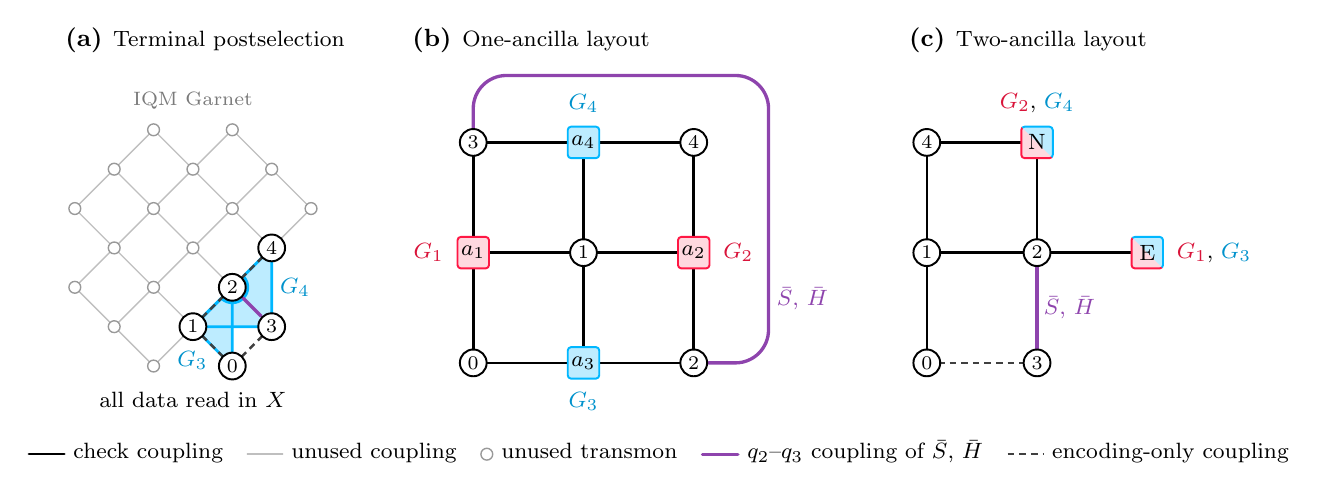
\begin{tikzpicture}[line cap=round,line join=round]

% panel grid centres A, B, C; titles sit at \yT, left-aligned (\tA, \tB, \tC
% from the centre) with the panel's ink; key row at \yK
\def\yT{2.62} \def\yK{-2.62}
\def\tA{-1.627} \def\tB{-2.18} \def\tC{-1.63}
\coordinate (A) at (1.77,0);    % Garnet lattice: 6*\gd = 3.00 cm wide
\coordinate (B) at (6.73,0);
\coordinate (C) at (12.49,0);

% ==================== (a) terminal postselection on IQM Garnet ====================
\begin{scope}[shift={(A)}]
  \GarnetCoords
  % X-type stabilizers that the terminal readout checks, shaded exactly as the
  % paper's current panel (a) (layout-figure/ancilla-layouts.tex; user, 2026-11-18):
  % Xtint fill, then the couplers, then 1pt XRim outlines. G3 = {q0,q1,q2};
  % G4 = {q1,q3,q4} has q2 on its long side and bypasses it. The dashed encoder
  % couplings, which share sides with the outlines, are drawn after them.
  \def\GthreePath{(q0) -- (q1) -- (q2) -- cycle}
  \def\GfourPath{(q3) -- (q4) -- ($(q2)+(45:\rd)$)
    arc[start angle=45,end angle=-135,radius=\rd] -- (q1) -- cycle}
  \path[fill=Xtint] \GthreePath; \path[fill=Xtint] \GfourPath;
  % each of the 30 couplers drawn once: grey unless the encoder (dashed) or the
  % logical gates (purple) use it, i.e. QB1-QB2, QB1-QB4, QB2-QB5, QB4-QB5, QB5-QB6
  \foreach \a/\b in \GarnetCouplers {%
    \pgfmathtruncatemacro{\key}{\a*100+\b}%
    \ifnum\key=102 \else\ifnum\key=104 \else\ifnum\key=205 \else\ifnum\key=405 \else
      \ifnum\key=506 \else \draw[unused] (QB\a) -- (QB\b);\fi\fi\fi\fi\fi}
  \path[draw=XRim,line width=1.0pt] \GthreePath; \path[draw=XRim,line width=1.0pt] \GfourPath;
  % the encoding circuit's couplers (layer 1: q0-q1, q2-q4; layer 2: q3-q0, q1-q2)
  \foreach \a/\b in {q0/q1,q2/q4,q3/q0,q1/q2}
    \draw[enc,dash phase=0.18pt,shorten <=\rq cm,shorten >=\rq cm] (\a) -- (\b);  % even ends on 0.37 cm
  \draw[gate,shorten <=\rq cm+0.5pt,shorten >=\rq cm+0.5pt] (q2) -- (q3);
  % stabilizer labels outside the shading: G3 below-left of q0-q1, G4 right of q3-q4
  \node[readout,text=XText,anchor=north east] at ($(q0)!0.5!(q1)+(-0.06,-0.06)$) {$G_3$};
  \node[readout,text=XText,anchor=west] at ($(q3)!0.5!(q4)+(0.10,0)$) {$G_4$};
  \node[readout,text=IdleQB!80!black,anchor=south,font=\scriptsize]
    at (0,3*\gd+0.32) {IQM Garnet};   % above QB20, QB17, clear of them
  \foreach \n in {3,7,8,9,10,11,12,13,14,15,16,17,18,19,20} \node[idleqb] at (QB\n) {};
  \DataNodes
  % every data qutrit is read in the X basis at the end of the sequence
  \node[readout,anchor=north] at (0,-\u-\lab) {all data read in $X$};   % level with (b)
\end{scope}
\Panel{$(A)+(\tA,\yT)$}{a}{Terminal postselection}

% ==================== (b) one-ancilla layout ====================
\begin{scope}[shift={(B)}]
  \OneAncCoords
  % long-range q2-q3 coupler of the logical gates, around the top-right corner
  \def\h{0.95}          % right side of the arc; its top runs 0.85 above the grid
  \draw[gate,rounded corners=0.42cm,shorten <=\rq cm+0.5pt,shorten >=\rq cm+0.5pt]
    (q3) -- (-\u,\u+0.85) -- (\u+\h,\u+0.85) -- (\u+\h,-\u) -- (q2);
  \node[readout,text=GateCol,anchor=west] at (\u+\h+0.10,-0.42*\u) {$\SH$};
  \foreach \a/\b in {a4/q3,a4/q1,a4/q4,a1/q3,a1/q1,a1/q0,a2/q4,a2/q1,a2/q2,a3/q0,a3/q1,a3/q2}
    \draw[used] (\a) -- (\b);
  \node[xsite] at (a4) {$a_4$}; \node[zsite] at (a1) {$a_1$};
  \node[zsite] at (a2) {$a_2$}; \node[xsite] at (a3) {$a_3$};
  \DataNodes
  \Readout{a4}{90}{\textcolor{XText}{$G_4$}}
  \Readout{a1}{180}{\textcolor{ZText}{$G_1$}}
  \Readout{a2}{0}{\textcolor{ZText}{$G_2$}}
  \Readout{a3}{270}{\textcolor{XText}{$G_3$}}
\end{scope}
\Panel{$(B)+(\tB,\yT)$}{b}{One-ancilla layout}

% ==================== (c) two-ancilla layout ====================
\begin{scope}[shift={(C)}]
  \BCoords
  % couplings: encoder only (dashed), check rounds (black), logical gates (purple)
  \draw[encedge,shorten <=\rq cm,shorten >=\rq cm] (q0) -- (q3);
  \foreach \a/\b in {q0/q1,q1/q2,q1/q4,q4/N,q2/N,q2/E} \draw[used] (\a) -- (\b);
  \draw[gate,shorten <=\rq cm+0.5pt,shorten >=\rq cm+0.5pt] (q2) -- (q3);
  \node[readout,text=GateCol,anchor=west] at ($(q2)!0.5!(q3)+(0.08,0)$) {$\SH$};
  \DualSite{N}{N}
  \DualSite{E}{E}
  \DataNodes
  \Readout{N}{90}{$\textcolor{ZText}{G_2},\,\textcolor{XText}{G_4}$}
  \Readout{E}{0}{$\textcolor{ZText}{G_1},\,\textcolor{XText}{G_3}$}
\end{scope}
\Panel{$(C)+(\tC,\yT)$}{c}{Two-ancilla layout}

% ==================== key (shared) ====================
% centred under the three panels as drawn
\path (current bounding box.west) coordinate (bbW) (current bounding box.east) coordinate (bbE);
\coordinate (bbM) at ($(bbW)!0.5!(bbE)$); \coordinate (keyY) at (0,\yK);
\node[anchor=base,inner sep=0pt,font=\footnotesize] at (bbM |- keyY) {%
  \KeyLine{used}\ check coupling\hspace{1.0em}%
  \KeyLine{unused}\ unused coupling\hspace{1.0em}%
  \KeyIdle\ unused transmon\hspace{1.0em}%
  \KeyLine{gate}\ $q_2$--$q_3$ coupling of $\SH$\hspace{1.0em}%
  \KeyLine{enc}\ encoding-only coupling};

\end{tikzpicture}
\end{document}
